%%%%%%%%%%%%%%%%%%%%%%%%%%%%%%%%%%%%%%%%%%%%%%%%%%%%%%%%%%%%%%%%%%%%%%%%%%
% PARTE 1: IMPOSTAZIONI GENERALI DEL DOCUMENTO
%%%%%%%%%%%%%%%%%%%%%%%%%%%%%%%%%%%%%%%%%%%%%%%%%%%%%%%%%%%%%%%%%%%%%%%%%%

\documentclass[11pt, a4paper]{report}

% LINGUA E CODIFICA
\usepackage[italian]{babel}
\usepackage[utf8]{inputenc}
\usepackage[T1]{fontenc}
\usepackage{lmodern}

% LAYOUT DI PAGINA E TIPOGRAFIA
\usepackage[margin=1.5cm, top=1.5cm, bottom=1.5cm]{geometry}
\usepackage{parskip}
\usepackage{microtype}

% GESTIONE DEI COLORI
\usepackage[table]{xcolor}

% MATEMATICA E SIMBOLI
\usepackage{amsmath, amssymb, amsfonts}
\usepackage{mathtools}
\usepackage{siunitx}

% BB OTTIMIZZAZIONE MATRICI LUNGHE PER LA STAMPA
\setlength{\arraycolsep}{10pt}
\usepackage{bm}

% GRAFICA, IMMAGINI E TABELLE
\usepackage{graphicx}
\usepackage{subcaption}
\graphicspath{{./Images/Tesina}}
\usepackage{float}
\usepackage{booktabs}
\usepackage{array}
\usepackage{multirow}
\usepackage{tabularx}

% DIAGRAMMI (TIKZ)
\usepackage{tikz}
\usetikzlibrary{shapes.geometric, arrows.meta, positioning, calc, quotes}
\usepackage{dirtree}

% LINK, RIFERIMENTI ED ELENCHI
\usepackage[unicode]{hyperref}
\hypersetup{
    colorlinks=true,
    linkcolor=black,
    urlcolor=blue,
    citecolor=blue,
    pdftitle={Tesina Industrial Robotic},
    pdfauthor={Francesco Lo Verde},
    pdfpagemode=FullScreen,
}
\usepackage{bookmark}
\usepackage[italian,capitalize]{cleveref}
\usepackage{enumitem}
\setlist{noitemsep}

% PERSONALIZZAZIONE TITOLI, TEOREMI E ALTRI PACCHETTI
\usepackage{titlesec}
\titleformat{\chapter}{\normalfont\huge\bfseries}{\thechapter.}{20pt}{\huge}
\titleformat{\section}{\normalfont\LARGE\bfseries}{\thesection}{1em}{}
\titleformat{\subsection}{\normalfont\Large\bfseries}{\thesubsection}{1em}{}
\titleformat{\subsubsection}{\normalfont\large\bfseries}{\thesubsubsection}{1em}{}
\titlespacing*{\chapter}{0pt}{0pt}{10pt}

\usepackage{comment}

%%%%%%%%%%%%%%%%%%%%%%%%%%%%%%%%%%%%%%%%%%%%%%%%%%%%%%%%%%%%%%%%%%%%%%%%%%
% PARTE 2: DEFINIZIONE DEGLI STILI PER IL CODICE
%%%%%%%%%%%%%%%%%%%%%%%%%%%%%%%%%%%%%%%%%%%%%%%%%%%%%%%%%%%%%%%%%%%%%%%%%%

\usepackage{listings}

% Definizione palette colori (ispirata a VS Code)
\definecolor{codepurple}{RGB}{204, 120, 220}
\definecolor{codecyan}{RGB}{78, 201, 176}
\definecolor{codeorange}{RGB}{206, 145, 120}
\definecolor{codegreen}{RGB}{106, 153, 85}
\definecolor{codeblue}{RGB}{86, 156, 214}
\definecolor{codegray}{rgb}{0.5, 0.5, 0.5}

% Stile di base comune a tutti i linguaggi
\lstdefinestyle{baseStyle}{
    backgroundcolor={},
    commentstyle=\color{codegreen}\itshape,
    stringstyle=\color{codeorange},
    basicstyle=\footnotesize\ttfamily,
    breaklines=true,
    breakatwhitespace=false,
    keepspaces=true,
    numbers=none,
    frame=none,
    showspaces=false,
    showstringspaces=false,
    showtabs=false,
    tabsize=4,
    captionpos=b,
    keywordstyle=\bfseries,
}

% Stile per BASH
\lstdefinestyle{bashStyle}{
    style=baseStyle,
    language=bash,
    keywordstyle={\color{codeblue}\bfseries},
    morekeywords={echo, ls, cd, mkdir, rm, cp, mv, sudo, apt-get, if, then, else, fi, for, in, do, done, while, case, esac, function},
}

% Stile per PYTHON
\lstdefinestyle{pythonStyle}{
    style=baseStyle,
    language=Python,
    keywordstyle=[1]{\color{codepurple}\bfseries},
    keywordstyle=[2]{\color{codeblue}},
    keywordstyle=[3]{\color{codecyan}\itshape},
    morekeywords={
        True, False, None, self, as, with, and, or, not, is, in,
        def, class, import, from, return, if, else, elif, for, while,
        try, except, finally, raise, pass, lambda, yield, global, nonlocal
    },
    morekeywords=[2]{
        print, len, range, int, str, float, list, dict, set, tuple, type,
        open, super, isinstance, zip, enumerate, map, filter
    },
    morekeywords=[3]{
        __init__, __str__, __repr__
    },
    sensitive=true,
}

% Stile per XML
\lstdefinestyle{XMLStyle}{
    style=baseStyle,
    language=XML,
    commentstyle=\color{codegreen},
    keywordstyle=\color{codeblue},
    morekeywords={version, encoding},
    otherkeywords={=},
    stringstyle=\color{codeorange},
    tagstyle=\color{codeblue},
    ndkeywordstyle=\color{codecyan},
}

\renewcommand{\DTcomment}[1]{%
  \dotfill\parbox[t]{7cm}{\raggedright\DTstylecomment{#1}}%
}

\author{Francesco Lo Verde}
\begin{document}
% --- Pagina del Titolo ---
\begin{titlepage}
    \centering

    % --- SEZIONE SUPERIORE: LOGO E UNIVERSITÀ ---
    
\includegraphics[width=0.35\textwidth]{Images/Tesina/LogoUnipg.png}\par\vspace{1.5cm}

    {\scshape\Large Università degli Studi di Perugia\par}

    \vfill % Aggiunge spazio flessibile

    % --- SEZIONE CENTRALE: TITOLI ---
    % Il titolo è lungo, quindi \huge è una buona dimensione.
    % Usiamo una minipage per controllare meglio la larghezza e prevenire una sillabazione sgradevole.
    \begin{minipage}{0.9\textwidth}
        \centering
        {\Huge \bfseries Sviluppo Di Un Package ROS Per La Modellazione E L'Analisi Cinematica Di Un Manipolatore RRP (3 DOF)\par}
    \end{minipage}

    \vspace{1cm}
    \rule{1\textwidth}{0.4pt} % Linea di separazione
    \vspace{1cm}

    {\LARGE \bfseries Corso di Industrial Robotics\par}

    \vfill % Aggiunge altro spazio flessibile

    % --- SEZIONE INFERIORE: AUTORE ---
    \begin{minipage}{0.7\textwidth}
    \begin{flushleft}
        \large
        \begin{tabular}{@{} l l}
            \multicolumn{2}{l}{\textbf{Studente}} \\
            \addlinespace[0.3em]
            Nome: & \textbf{Francesco Lo Verde} \\
            Email: & \texttt{francesco.loverde@studenti.unipg.it} \\
        \end{tabular}
    \end{flushleft}
    \end{minipage}

    \vspace{1.5cm}

    % --- PIÈ DI PAGINA: ANNO ACCADEMICO ---
    {\large Anno Accademico 2025-2026\par}
    %\vspace{0.5cm}
    %{\small Data ultimo aggiornamento: \today\par}

\end{titlepage}

\restoregeometry

% --- Indice ---
\tableofcontents
\cleardoublepage

%%%%%%%%%%%%%%%%%%%%%%%%%%%%%%%%%%%%%%%%%%%%%%%%%%%%%%%%%%%%%%%%%%%%%%%%%%
% INIZIO CAPITOLO 1
%%%%%%%%%%%%%%%%%%%%%%%%%%%%%%%%%%%%%%%%%%%%%%%%%%%%%%%%%%%%%%%%%%%%%%%%%%
\chapter{Introduzione}
\section{Obiettivi Del Progetto}
Questo report documenta lo sviluppo di un pacchetto \textbf{Robot Operating System (ROS)} denominato \texttt{manipolatoreRRP}, mirato alla simulazione, al controllo e all'analisi cinematica di un manipolatore robotico antropomorfo seriale a tre gradi di libertà (RRP - Rotatorio, Rotatorio, Prismatico) con end-effector fisso orientato verso il basso.

L'obiettivo primario è la creazione di un ambiente virtuale integrato che permetta di validare la cinematica diretta (calcolata analiticamente tramite la convenzione di Denavit-Hartenberg) e di implementare la cinematica inversa, il controllo dei limiti fisici dei giunti e l'analisi delle singolarità geometriche.

Gli obiettivi specifici del progetto sono i seguenti:
\begin{itemize}
    \item \textbf{Modellazione Parametrica:} Sviluppare un modello geometrico e visivo accurato del manipolatore in formato \texttt{XACRO} (\textit{XML Macro}), leggendo i parametri strutturali direttamente da un file di configurazione centrale in formato \texttt{YAML}.

    \item \textbf{Integrazione dell'Ambiente 3D:} Configurare l'ambiente di visualizzazione tridimensionale \texttt{RViz} per ispezionare lo stato del robot e validare visivamente i movimenti sia tramite interfaccia grafica a slider (\texttt{joint\_state\_publisher\_gui}) sia tramite l'invio di comandi diretti da terminale.

    \item \textbf{Esecuzione Condizionale e Flessibile:} Realizzare un file di lancio (\texttt{.launch}) in grado di orchestrare l'avvio dei nodi ROS e di offrire due modalità operative distinte (manuale interattiva con GUI o automatica/analitica da riga di comando) tramite parametri condizionali.

    \item \textbf{Analisi Cinematica e Controllo:} Sviluppare un'architettura software in Python per calcolare in tempo reale la cinematica diretta e inversa, verificare l'ammissibilità dei target all'interno del workspace operativo, monitorare la vicinanza a configurazioni singolari mediante lo studio del determinante Jacobiano e intercettare le trasformazioni spaziali tramite un listener \texttt{TF2}.
\end{itemize}

\newpage
\subsection{Il Manipolatore Antropomorfo RRP}
La struttura del manipolatore sviluppato si basa su una catena cinematica seriale a tre gradi di libertà principali più un End-Effector fisso, progettata per coniugare pulizia geometrica e realismo meccanico. Per evitare l'effetto visivo irrealistico dello scorrimento dell'intera guida lineare, la scatola del giunto prismatico è solidale al braccio precedente, consentendo solo allo stelo interno di scorrere fisicamente. Ciascun giunto rotatorio è inoltre protetto visivamente da sfere estetiche per eliminare vuoti d'aria o compenetrazioni geometriche.
\begin{figure}[h!]
    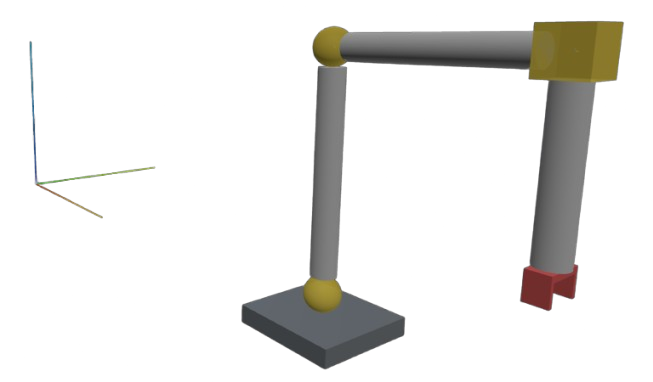
\includegraphics[width=\linewidth]{isoViewNoBg.png}
    \caption{Modello 3D del manipolatore RRP.}
    \label{fig:modello_robot}
\end{figure}

La catena cinematica del manipolatore è definita da:
\begin{itemize}
    \item \textbf{Base fissa:} Un blocco rettangolare ancorato a terra con un offset di $2.0$ metri lungo l'asse $X$ rispetto al frame globale \texttt{world}.
    \item \textbf{Giunto 1 (\texttt{giunto1}):} Giunto rotatorio attorno all'asse verticale $Z$, posizionato sulla faccia superiore della base.
    \item \textbf{Link 1 (\texttt{RF0}):} Colonna cilindrica di lunghezza $l_1$ che si sviluppa verticalmente lungo l'asse $Z$.
    \item \textbf{Giunto 2 (\texttt{giunto2}):} Giunto rotatorio attorno all'asse trasversale locale $Y$, con limiti impostati per prevenire auto-collisioni con la colonna.
    \item \textbf{Link 2 (\texttt{RF1}):} Braccio cilindrico di lunghezza $l_2$ che si estende in direzione radiale e termina con il box cubico della guida prismatica.
    \item \textbf{Giunto 3 (\texttt{giunto3}):} Giunto prismatico lineare che scorre lungo l'asse verticale locale del braccio.
    \item \textbf{Link 3 (\texttt{RF2}):} Asta cilindrica interna di lunghezza $l_3$ che scorre dentro la scatola di guida.
    \item \textbf{End-Effector (\texttt{endEffector}):} Pinza fissa solidale all'estremità inferiore dell'asta, ruotata di $180^\circ$ per operare sul piano del tavolo di lavoro ($Z=0$).
\end{itemize}

%%%%%%%%%%%%%%%%%%%%%%%%%%%%%%%%%%%%%%%%%%%%%%%%%%%%%%%%%%%%%%%%%%%%%%%%%%
% INIZIO CAPITOLO 2
%%%%%%%%%%%%%%%%%%%%%%%%%%%%%%%%%%%%%%%%%%%%%%%%%%%%%%%%%%%%%%%%%%%%%%%%%%

\chapter{Strumenti E Architettura Del Sistema}
\label{chap:strumenti_tecnologie}

\section{Il Framework ROS (Robot Operating System)}
L'infrastruttura software sfrutta le potenzialità di \textbf{ROS (Robot Operating System) Noetic}. La modularità del framework ha consentito di separare nettamente la definizione geometrica del manipolatore dalla logica algoritmica di controllo e calcolo cinematico.

L'interconnessione tra i nodi avviene dinamicamente mediante la pubblicazione e sottoscrizione sul topic \texttt{/joint\_states} e l'interrogazione dell'albero delle trasformazioni (\texttt{/tf}). A seconda dell'argomento di lancio impostato dall'utente, il sistema si adatta a due diverse topologie di comunicazione (Grafo ROS).

\begin{figure}[htbp] % [htbp] offre in genere una gestione migliore del posizionamento rispetto a [h!]
    \centering
    \begin{subfigure}[b]{0.9\textwidth}
        \centering
        % Se necessario, ripristina il percorso completo: Images/Tesina/rqtGraphWithGUI.png
        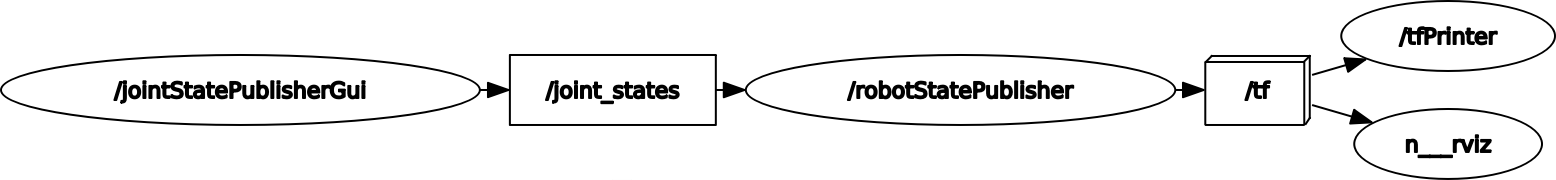
\includegraphics[width=\textwidth]{Images/Tesina/rqtGraphWithGUI.png}
        \caption{Configurazione con interfaccia grafica abilitata (\texttt{gui:=True}).}
        \label{fig:graph_gui}
    \end{subfigure}

    \vspace{0.5cm} % Sostituito \hfill con uno spazio verticale per separare le figure sovrapposte

    \begin{subfigure}[b]{0.9\textwidth}
        \centering
        % Se necessario, ripristina il percorso completo: Images/Tesina/rqtGraphNoGUI.png
        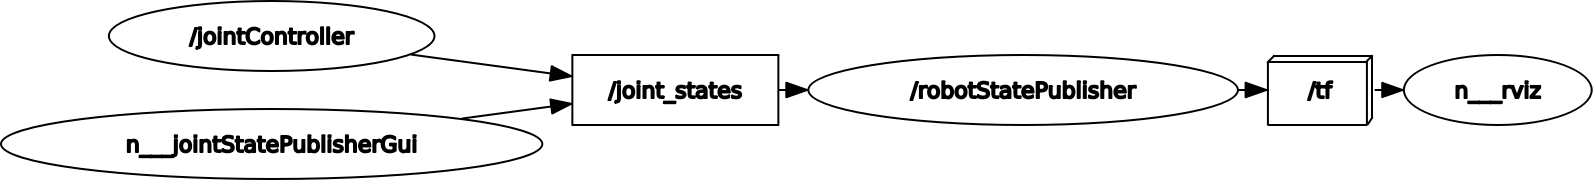
\includegraphics[width=\textwidth]{Images/Tesina/rqtGraphNoGUI.png}
        \caption{Configurazione con controllo da terminale (\texttt{gui:=False}).}
        \label{fig:graph_controller}
    \end{subfigure}
    \caption{Grafo delle comunicazioni tra nodi e topic generato con \texttt{rqt\_graph}.}
    \label{fig:ros_graphs}
\end{figure}

\subsection{Modellazione Parametrica: XACRO e URDF}
Il robot è descritto in formato \texttt{XACRO} all'interno del file \texttt{manipolatoreRRP.urdf.xacro}. Questa scelta consente una modellazione flessibile: le dimensioni fisiche della base, dei link ($l_1, l_2, l_3$) e dell'end-effector non sono cablate nel codice XML, ma caricate dinamicamente dal file YAML di configurazione.

L'albero cinematico strutturato nel file XML definisce la gerarchia dei corpi rigidi (\textit{Link}) e le limitazioni fisiche dei giunti (\textit{Joint}):
\begin{itemize}
    \item \textbf{Giunti Rotatori (\texttt{revolute}):} Definiti per il movimento azimutale della base e ddella spalla, con limiti in radianti.
    \item \textbf{Giunto Prismatico (\texttt{prismatic}):} Configurato per lo scorrimento lineare dell'asta, con limiti di corsa compresi tra $0$ e $l_3$.
    \item \textbf{Giunti Fissi (\texttt{fixed}):} Utilizzati per ancorare stabilmente il manipolatore al terreno (\texttt{world} $\rightarrow$ \texttt{base}) e per posizionare l'end-effector sulla punta dell'asta telescopica (\texttt{RF2} $\rightarrow$ \texttt{endEffector}).
\end{itemize}
\newpage
\subsection{Gestione Delle Trasformazioni Spaziali (TF2)}
La gestione e l'aggiornamento dei sistemi di coordinate locali (\textit{frame}) sono affidati alla libreria \textbf{TF2}. Il nodo \texttt{robot\_state\_publisher} riceve lo stato istantaneo dei giunti dal topic \texttt{/joint\_states} e, combinandolo con la struttura definita nell'URDF, calcola la catena cinematica completa.

L'albero dei frame risultante (mostrato in Figura~\ref{fig:tf_tree}) descrive la sequenza esatta di coordinate dall'origine globale fissa (\texttt{world}) fino alla flangia operativa della pinza (\texttt{endEffector}):

\begin{figure}[H]
    \centering
    % Dopo roslaunch manipolatoreRRP manipolatoreRRP.launch, in un'altro terminale, eseguire il comando:
    % source ~/catkin_ws/devel/setup.bash
    % rosrun tf2_tools view_frames.py
    % \includegraphics[width=0.45\textwidth]{tf_tree_rrp.png}
    \caption{Albero delle trasformazioni spaziali (TF Tree) del manipolatore RRP.}
    \label{fig:tf_tree}
\end{figure}

\newpage
\section{Struttura del Package \texttt{manipolatoreRRP}}
Il progetto è strutturato come un package ROS standard denominato \texttt{manipolatoreRRP}. Di seguito viene riportato l'albero effettivo dei file che compongono l'architettura:

\dirtree{%
.1 manipolatoreRRP.
.2 CMakeLists.txt\DTcomment{File di configurazione ROS}.
.2 package.xml\DTcomment{File delle dipendenze ROS}.
.2 config.
.3 robotParameters.yaml\DTcomment{Parametri fisici del robot}.
.2 launch.
.3 manipolatoreRRP.launch\DTcomment{File di avvio}.
.2 scripts.
.3 directKinematics.py\DTcomment{Script per la cinematica diretta}.
.3 inverseKinematics.py\DTcomment{Script per la cinematica inversa}.
.3 jointController.py\DTcomment{Script per il controllo dei giunti}.
.3 kinematicsUtils.py\DTcomment{File di utilità per la cinematica}.
.3 tfPrinter.py\DTcomment{Node listener per la stampa della posa}.
.2 urdf.
.3 manipolatoreRRP.urdf.xacro\DTcomment{Descrizione geometrica}.
}

\subsection{Infrastruttura di Avvio: \texttt{manipolatoreRRP.launch}}
Il file di lancio centralizza l'inizializzazione dell'intero workspace e implementa un controllo condizionale basato sulla variabile \texttt{gui} (valore di default: \texttt{True}):

\begin{enumerate}
    \item \textbf{Inizializzazione dei Parametri:} Carica sul Parameter Server di ROS le variabili geometriche definite in \texttt{robotParameters.yaml}, esponendo chiavi globali come \texttt{/l1}, \texttt{/l2}, \texttt{/l3} e \texttt{/worldBase}.

    \item \textbf{Generazione del Modello:} Invoca lo strumento \texttt{xacro} per compilare a tempo di esecuzione il file \texttt{manipolatoreRRP.urdf.xacro} in un file URDF standard, memorizzandolo nel parametro \texttt{robot\_description}.

    \item \textbf{Bivio Operativo (Condizionale):}
    \begin{itemize}
        \item \textbf{Se \texttt{gui:="True"}:} Avvia il nodo \texttt{joint\_state\_publisher\_gui}, che genera un'interfaccia a cursori per comandare manualmente i giunti. Parallelamente, avvia lo script \texttt{tfPrinter.py} per monitorare le matrici omogenee di trasformazione.
        \item \textbf{Se \texttt{gui:="False"}:} Esclude la GUI e il listener TF, avviando al loro posto il nodo interattivo \texttt{jointController.py} per l'input di coordinate cinematiche dirette o inverse da terminale.
    \end{itemize}

    \item \textbf{Aggiornamento TF e RViz:} In entrambe le modalità, il nodo \texttt{robot\_state\_publisher} elabora i dati di giunto pubblicati su \texttt{/joint\_states} per aggiornare l'albero delle trasformazioni dinamiche, mentre \texttt{rviz} carica una configurazione preimpostata per mostrare il modello 3D in tempo reale.
\end{enumerate}

\subsection{Cartella Script Python (\texttt{scripts/})}
La logica algoritmica e di controllo del manipolatore è suddivisa in cinque script specializzati:

\begin{itemize}
    \item \textbf{\texttt{kinematicsUtils.py}:} Funge da libreria centrale di supporto. Gestisce il caricamento dei parametri fisici dal ROS Parameter Server, implementa le funzioni di saturazione (\textit{clamping}) dei giunti (\texttt{checkJointLimits}) in base alle specifiche di progetto, crea i messaggi di tipo \texttt{JointState} e calcola la vicinanza a singolarità strutturali (\texttt{checkSingularity}) restituendo il determinante Jacobiano associato.

    \item \textbf{\texttt{directKinematics.py}:} Implementa l'algoritmo di calcolo della cinematica diretta. Utilizza una tabella di Denavit-Hartenberg basata sui parametri dimensionali del robot per calcolare le matrici omogenee di giunto e ricavare la posa tridimensionale complessiva dell'end-effector rispetto al frame globale \texttt{world}.
    \newpage
    \item \textbf{\texttt{inverseKinematics.py}:} Risolve per via geometrico-analitica il problema cinematico inverso. Ricevuto un target cartesiano $(x, y, z)$ in coordinate mondo, calcola le variabili di giunto $q_1, q_2, q_3$ discriminando le configurazioni a gomito alto (\textit{elbow up}) e gomito basso (\textit{elbow down}) ed escludendo le soluzioni matematiche che superano i limiti fisici del robot.

    \item \texttt{\textbf{jointController.py}} (Attivo con \texttt{gui:=False}): Costituisce l'interfaccia interattiva a riga di comando per l'utente. Permette di selezionare ciclicamente la modalità di inserimento (cinematica diretta per impostare i giunti, o cinematica inversa per digitare un target cartesiano), esegue i controlli preventivi del workspace tramite la libreria di utilità e aggiorna la visualizzazione in RViz pubblicando i nuovi valori sul topic \texttt{/joint\_states} ad una frequenza di $50$ Hz.

    \item \texttt{\textbf{tfPrinter.py}} (Attivo con \texttt{gui:=True}): Implementa un TF Listener che interroga l'albero delle trasformazioni ad una frequenza costante di $1$ Hz. Estrae la traslazione e il quaternione di rotazione tra i frame \texttt{world} ed \texttt{endEffector}, li converte in una matrice omogenea di trasformazione $4 \times 4$ e la stampa formattata sul terminale.
\end{itemize}


%%%%%%%%%%%%%%%%%%%%%%%%%%%%%%%%%%%%%%%%%%%%%%%%%%%%%%%%%%%%%%%%%%%%%%%%%%
% INIZIO CAPITOLO 3
%%%%%%%%%%%%%%%%%%%%%%%%%%%%%%%%%%%%%%%%%%%%%%%%%%%%%%%%%%%%%%%%%%%%%%%%%%

\chapter{Modellazione Cinematica Del Manipolatore}
\label{chap:modellazione_cinematica}

La modellazione cinematica descrive matematicamente le relazioni geometriche tra le coordinate dei giunti di un manipolatore e la posa (posizione e orientamento) dell'organo terminale nello spazio tridimensionale. Per l'analisi del manipolatore a tre gradi di libertà (RRP) in oggetto, si è adottato il formalismo cinematico basato sulla convenzione di Denavit-Hartenberg.

La \textbf{convenzione di Denavit-Hartenberg (DH)} definisce un metodo sistematico per associare sistemi di riferimento locali (\(RF_i\)) a ciascun link \(i\) di una catena cinematica seriale aperta, consentendo di descrivere la trasformazione spaziale tra frame adiacenti tramite quattro parametri geometrici fondamentali:
\begin{itemize}
    \item \(\bm{\theta_i}\) (\textit{Angolo di giunto}): Rotazione attorno all'asse \(Z_{i-1}\) necessaria per allineare l'asse \(X_{i-1}\) con l'asse \(X_i\).
    \item \(\bm{d_i}\) (\textit{Offset del link}): Traslazione lungo l'asse \(Z_{i-1}\) per portare l'origine di \(RF_{i-1}\) sul piano \(X_i Y_i\).
    \item \(\bm{a_i}\) (\textit{Lunghezza del link}): Traslazione lungo il nuovo asse \(X_i\) per far coincidere l'origine traslata con l'origine effettiva di \(RF_i\).
    \item \(\bm{\alpha_i}\) (\textit{Torsione del link}): Rotazione attorno al nuovo asse \(X_i\) necessaria per allineare l'asse \(Z_{i-1}\) con l'asse \(Z_i\).
\end{itemize}

Nel caso di giunti rotatori, la variabile di giunto è l'angolo \(\theta_i = q_i\), mentre per i giunti prismatici la variabile è l'estensione lineare \(d_i\). La composizione dei quattro movimenti elementari associati a questi parametri si traduce nella matrice di trasformazione omogenea standard \(^{i-1}T_i\):
\[
\scalebox{0.8}{$
    ^{i-1}T_i =
    \begin{pmatrix}
        \cos\theta_i & -\sin\theta_i\cos\alpha_i & \sin\theta_i\sin\alpha_i & a_i\cos\theta_i \\
        \sin\theta_i & \cos\theta_i\cos\alpha_i & -cos\theta_i\sin\alpha_i & a_i\sin\theta_i \\
        0 & \sin\alpha_i & \cos\alpha_i & d_i \\
        0 & 0 & 0 & 1
    \end{pmatrix}
$}
\]

Applicando questa convenzione al manipolatore RRP in esame, si definisce la tabella dei parametri DH riportata in Tabella~\ref{tab:dh_rrp}. I parametri costanti integrano rigorosamente gli offset strutturali dovuti alle sfere estetiche dei giunti (di raggio \(r_{g} = 0.05\) m) e alla scatola di guida cubica del giunto prismatico (di lato \(b = 0.10\) m).

\begin{table}[h!]
    \centering
    \resizebox{0.6\textwidth}{!}{
        \begin{tabular}{|c|c|c|c|c|c|}
            \hline
            \textbf{Trasformazione} & \textbf{\# Link} & \(\bm{\theta_i}\) & \(\bm{d_i}\) & \(\bm{\alpha_i}\) & \(\bm{a_i}\) \\
            \hline
            $RF_{0} \to RF_{1}$ & 1 & $q_{1}$ & $d_{1} = 3 r_{g} + l_1$ & $-\frac{\pi}{2}$ & 0 \\
            \hline
            $RF_{1} \to RF_{2}$ & 2 & $q_{2}$ & 0 & $\frac{\pi}{2}$ & $a_{2} = r_{g} + l_2 + \frac{b}{2}$ \\
            \hline
            $RF_{2} \to RF_{EE}$ & 3 & 0 & $d_{3} = q_3 - \left(l_3 + \frac{b}{2}\right)$ & $-\pi$ & 0\\
            \hline
        \end{tabular}
    }
    \caption{Parametri di Denavit-Hartenberg per il manipolatore RRP.}
    \label{tab:dh_rrp}
\end{table}

\begin{itemize}
    \item \textbf{Giunto 1 e Link 1:} Rappresenta la rotazione azimutale attorno all'asse verticale \(Z_0\). L'offset verticale complessivo \(d_1 = 0.70\) m tiene conto dello sviluppo del cilindro (\(l_1 = 0.55\) m) e del raggio delle sfere di accoppiamento per eliminare discontinuità geometriche. La torsione \(\alpha_1 = -\pi/2\) orienta l'asse \(Z_1\) in direzione ortogonale per il giunto successivo.

    \item \textbf{Giunto 2 e Link 2:} Costituisce idella spalla del robot. L'asse di rotazione è \(Y_1\) locale. L'estensione orizzontale del braccio \(a_2 = 0.55\) m comprende la lunghezza del link cilindrico (\(l_2 = 0.45\) m), il raggio della sfera di spalla e metà del lato del box prismatico (\(b/2 = 0.05\) m), posizionando l'origine del frame della guida all'estremità fisica del braccio.

    \item \textbf{Giunto 3 e Link 3:} Rappresenta lo stelo prismatico scorrevole. Poiché la guida lineare non ruota rispetto al braccio precedente, l'angolo \(\theta_3\) è nullo. L'offset \(d_3\) è guidato dalla coordinata lineare \(q_3\). Quando il giunto si trova a riposo (\(q_3 = 0\)), l'asse si estende completamente verso il basso con un offset negativo pari alla somma della lunghezza dell'asta (\(l_3 = 0.35\) m) e di metà del box di guida (\(b/2 = 0.05\) m), ovvero \(d_3 = -0.40\) m. La torsione \(\alpha_3 = -\pi\) ruota il frame finale di \(180^\circ\) attorno all'asse \(X\) per orientare l'end-effector verso il piano di lavoro.
\end{itemize}

La cinematica diretta del manipolatore esprime la posa del frame dell'end-effector (\(RF_{EE}\)) rispetto al frame alla base della colonna (\(RF_0\)), ed è ricavata dal prodotto ordinato delle matrici di trasformazione omogenea locali:
\[
    ^{0}T_{EE} = {^{0}T_1}(q_1) \cdot {^{1}T_2}(q_2) \cdot {^{2}T_{EE}}(q_3)
\]

\newpage
\section{Modello Nell'Ambiente ROS}
\label{sec:implementazione_ros}

La rappresentazione del modello cinematico all'interno dell'ambiente ROS Noetic è realizzata tramite lo standard XML \texttt{URDF}, arricchito con le macro \texttt{XACRO} per garantire la modularità geometrica.

Mentre il modello matematico di Denavit-Hartenberg descrive le trasformazioni cinematiche tramite assi e origini calcolati per astrazione algebrica, lo standard URDF richiede una modellazione basata sulla gerarchia fisica di link (corpi rigidi con proprietà visive, materiali e dimensionali) e giunti (elementi di accoppiamento e vincolo spaziale).

Per implementare fedelmente il meccanismo telescopico del giunto prismatico, la scatola cubica di guida (\texttt{boxSize}) è stata definita all'interno delle proprietà visive dello stesso link padre (\texttt{RF1}), mentre solo l'asta interna cilindrica (\texttt{RF2}) è stata associata al giunto lineare. A titolo di esempio, il listato seguente illustra l'implementazione XML del giunto prismatico \texttt{giunto3} e del relativo link figlio scorrevole \texttt{RF2}:

\begin{lstlisting}[style=XMLStyle]
<!-- Giunto 3 (Prismatico - Scorrimento su asse Z locale) -->
<joint name="giunto3" type="prismatic">
    <parent link="RF1"/>
    <child link="RF2"/>
    <!-- Posizionamento sull'asse della guida cubica all'estremita del braccio -->
    <origin xyz="${jointRadius + l2 + (boxSize/2)} 0 0" rpy="0 0 0"/>
    <axis xyz="0 0 1"/>
    <limit effort="100" velocity="1.0" lower="0" upper="${l3}"/>
</joint>

<!-- Link 2 (Asta cilindrica prismatica) -->
<link name="RF2">
    <visual>
        <!-- Spostato in basso di meta box + meta lunghezza link per lo scorrimento -->
        <origin xyz="0 0 -${(l3/2) + (boxSize/2)}" rpy="0 0 0"/>
        <geometry>
                <cylinder radius="${linkRadius}" length="${l3}" />
        </geometry>
        <material name="linkColor"/>
    </visual>
</link>
\end{lstlisting}

\subsection{Visualizzazione Della Catena Cinematica}
\label{subsec:catena_cinematica_world}

All'interno dell'ambiente ROS, la topologia gerarchica del robot viene convertita in un albero di sistemi di riferimento dinamici gestito dalla libreria \texttt{tf2}.

A differenza di una catena cinematica ancorata all'origine, in questo progetto si è modellato l'ancoraggio strutturale del robot rispetto al frame globale \texttt{world} tramite un offset rigido posizionato sul piano cartesiano del tavolo da lavoro:
\begin{enumerate}
    \item \textbf{Frame \texttt{world}:} È l'origine fissa del sistema di coordinate globali di simulazione.
    \item \textbf{Base del manipolatore:} Un giunto fisso denominato \texttt{giuntoWorld} fissa il link \texttt{base} a una distanza di $2.0$ metri lungo l'asse $X$ rispetto al frame \texttt{world}, con un orientamento coincidente.
    \item \textbf{Origine della catena mobile (\texttt{RF0}):} Il giunto rotatorio principale \texttt{giunto1} connette la base al primo link mobile della colonna verticale. Esso presenta un offset costante lungo $Z$ pari all'altezza della base stessa (\texttt{baseHeight} = $0.05$ m). La sequenza di frame dinamici si sviluppa pertanto secondo lo schema:
    \[
        \texttt{world} \xrightarrow{\text{Fisso (2.0, 0, 0)}} \texttt{base} \xrightarrow{\text{giunto1 (0, 0, 0.05)}} \texttt{RF0} \xrightarrow{\text{giunto2}} \texttt{RF1} \xrightarrow{\text{giunto3}} \texttt{RF2}
    \]
    \item \textbf{Frame \texttt{endEffector}:} All'estremità inferiore dell'asta scorrevole \texttt{RF2} è applicato il frame operativo finale tramite il giunto fisso \texttt{giuntoEE}. Questo frame descrive la posa del \textit{Tool Center Point} (TCP) della pinza bidito e ne imposta l'orientamento di $180^\circ$ attorno all'asse $X$, proiettandone l'azione verso il piano del tavolo di lavoro.
\end{enumerate}


%%%%%%%%%%%%%%%%%%%%%%%%%%%%%%%%%%%%%%%%%%%%%%%%%%%%%%%%%%%%%%%%%%%%%%%%%%
% INIZIO CAPITOLO 4
%%%%%%%%%%%%%%%%%%%%%%%%%%%%%%%%%%%%%%%%%%%%%%%%%%%%%%%%%%%%%%%%%%%%%%%%%%

\chapter{Analisi Della Trasformazione Cinematica}
\label{chap:analisi_cinematica}

La validazione analitica e numerica rappresenta una fase fondamentale per assicurare che il modello cinematico implementato in simulazione corrisponda coerentemente alle equazioni geometriche teoriche. A tale scopo, è stato sviluppato uno script di analisi in Python che interroga in tempo reale le trasformazioni fornite dal sistema di coordinate di ROS.

\section{Acquisizione Della Posa}
\label{sec:acquisizione_dati}

L'acquisizione in tempo reale delle relazioni spaziali tra i frame è implementata nello script \texttt{tfPrinter.py}, il quale sfrutta le classi di comunicazione fornite dalla libreria \texttt{tf2\_ros}. All'interno del nodo viene istanziato un buffer di memoria (\texttt{tf2\_ros.Buffer}) e un listener (\texttt{tf2\_ros.TransformListener}) adibito alla ricezione delle trasformazioni.

Il nodo esegue un loop periodico con una frequenza di aggiornamento pari a $1$ Hz. Ad ogni iterazione, lo script invoca la funzione:
\begin{lstlisting}[language=Python]
dataTF = tf_buffer.lookup_transform('world', 'endEffector', rospy.Time(0))
\end{lstlisting}
Questa istruzione interroga il sistema TF2 per ricavare la posa del frame \texttt{endEffector} rispetto al frame di riferimento globale \texttt{world}. L'oggetto restituito racchiude i dati geometrici in forma di coordinate cartesiane del vettore di traslazione \((x, y, z)\) e di quaternione unitario di rotazione \((q_x, q_y, q_z, q_w)\).

\subsection{Conversione In Matrice Omogenea 4x4}
\label{subsec:conversione_matrice}

Per abilitare il confronto analitico, la combinazione di traslazione e quaternione viene convertita in una singola matrice di trasformazione omogenea di dimensione $4 \times 4$. Nello script \texttt{tfPrinter.py} la conversione è effettuata chiamando la funzione \texttt{quaternion\_matrix()} del modulo \texttt{tf.transformations}:
\begin{enumerate}
    \item Il quaternione \(\mathbf{q}\) viene convertito in una matrice di rotazione ortonormale \(R \in \mathbb{R}^{3 \times 3}\).
    \item La matrice omogenea complessiva $^{world}T_{endEffector}$ viene costruita associando la matrice di rotazione \(R\) e il vettore di traslazione \(\mathbf{p} = [p_x, p_y, p_z]^T\) secondo lo schema a blocchi standard:
    \[
        ^{world}T_{endEffector} =
        \begin{pmatrix}
            r_{11} & r_{12} & r_{13} & p_x \\
            r_{21} & r_{22} & r_{23} & p_y \\
            r_{31} & r_{32} & r_{33} & p_z \\
            0 & 0 & 0 & 1
        \end{pmatrix}
    \]
\end{enumerate}

La matrice così assemblata descrive in modo univoco sia l'orientamento della pinza (colonne della matrice di rotazione, le quali rappresentano i versori locali degli assi dell'end-effector espressi in coordinate mondo) sia la posizione del TCP nello spazio cartesiano globale.
\newpage

\section{Validazione Della Posa Nella Configurazione Di Home}
\label{sec:validazione_posa}

La validazione numerica del sistema è stata condotta ponendo il manipolatore nella configurazione geometrica fondamentale di "Home", caratterizzata da valori di giunto nulli:
\[
    \mathbf{q}_{home} = [q_1, q_2, q_3]^T = [0.0 \text{ rad}, 0.0 \text{ rad}, 0.0 \text{ m}]^T
\]

All'avvio del sistema tramite il file \texttt{manipolatoreRRP.launch} con interfaccia grafica attiva, i giunti vengono posizionati di default a zero. In questa condizione, lo script \texttt{tfPrinter.py} intercetta la trasformazione spaziale e produce a terminale il seguente output:

\begin{verbatim}
-----------------------------------------------------
Trasformazione Da 'endEffector' a 'world'

Timestamp: 1784553396.6524231

Traslazione (x, y, z):
         x: 2.5501
         y: 0.0000
         z: 0.3501

Quaternione (Rotazione x, y, z, w) :
         x: 1.0000
         y: -0.0000
         z: 0.0001
         w: 0.0000

Matrice Trasformazione Omogenea world - endEffector:

[[ 1.   -0.    0.    2.55]
 [ 0.   -1.   -0.    0.  ]
 [ 0.    0.   -1.    0.35]
 [ 0.    0.    0.    1.  ]]
-----------------------------------------------------
\end{verbatim}

\subsection{Correlazione Analitica Con Il Modello Geometrico}
\label{subsec:discussione_risultati}

Per validare rigorosamente la correttezza della catena cinematica, si confrontano i valori misurati a terminale con la risoluzione analitica basata sulle matrici di Denavit-Hartenberg. Le trasformazioni geometriche globali che collegano il frame \texttt{world} al frame \texttt{endEffector} sono descritte dall'espressione:
\[
    ^{world}T_{endEffector} = {^{world}T_{base}} \cdot {^{base}T_0} \cdot {^{0}T_1}(q_1) \cdot {^{1}T_2}(q_2) \cdot {^{2}T_{EE}}(q_3)
\]

Con i parametri geometrici estratti dal Parameter Server di ROS (\(worldBase = 2.0\) m, \(baseHeight = 0.05\) m, \(d_1 = 0.70\) m, \(a_2 = 0.55\) m, \(d_3 = q_3 - 0.40\) m), si impostano i valori della posa di Home (\(q_1 = q_2 = q_3 = 0\)).

Le matrici omogenee elementari assumono la forma:
\[
    ^{world}T_{base} = \begin{pmatrix} 1 & 0 & 0 & 2.0 \\ 0 & 1 & 0 & 0 \\ 0 & 0 & 1 & 0 \\ 0 & 0 & 0 & 1 \end{pmatrix}, \quad
    ^{base}T_{0} = \begin{pmatrix} 1 & 0 & 0 & 0 \\ 0 & 1 & 0 & 0 \\ 0 & 0 & 1 & 0.05 \\ 0 & 0 & 0 & 1 \end{pmatrix}
\]
\[
    ^{0}T_{1} = \begin{pmatrix} 1 & 0 & 0 & 0 \\ 0 & 0 & 1 & 0 \\ 0 & -1 & 0 & 0.70 \\ 0 & 0 & 0 & 1 \end{pmatrix}, \quad
    ^{1}T_{2} = \begin{pmatrix} 1 & 0 & 0 & 0.55 \\ 0 & 0 & -1 & 0 \\ 0 & 1 & 0 & 0 \\ 0 & 0 & 0 & 1 \end{pmatrix}, \quad
    ^{2}T_{EE} = \begin{pmatrix} 1 & 0 & 0 & 0 \\ 0 & -1 & 0 & 0 \\ 0 & 0 & -1 & -0.40 \\ 0 & 0 & 0 & 1 \end{pmatrix}
\]

Moltiplicando in sequenza le trasformazioni relative alla sola catena mobile del manipolatore (\(^{0}T_{EE} = {^{0}T_1} \cdot {^{1}T_2} \cdot {^{2}T_{EE}}\)), si ottiene la matrice omogenea locale:
\[
    ^{0}T_{EE} = \begin{pmatrix} 1 & 0 & 0 & 0.55 \\ 0 & -1 & 0 & 0 \\ 0 & 0 & -1 & 0.30 \\ 0 & 0 & 0 & 1 \end{pmatrix}
\]

Infine, applicando la rototraslazione iniziale rispetto all'origine globale (\(^{world}T_{endEffector} = {^{world}T_{base}} \cdot {^{base}T_0} \cdot {^{0}T_{EE}}\)), si giunge alla matrice globale analitica:
\[
    ^{world}T_{endEffector} =
    \begin{pmatrix}
        1 & 0 & 0 & 2.55 \\
        0 & -1 & 0 & 0.00 \\
        0 & 0 & -1 & 0.35 \\
        0 & 0 & 0 & 1
    \end{pmatrix}
\]

\subsubsection{Analisi del Vettore di Posizione e d'Orientamento}

Il confronto tra il calcolo analitico e l'output dello script rivela un allineamento rigoroso della posa:
\begin{itemize}
    \item \textbf{Coordinata $X$ ($2.55$ m):} È la somma esatta della traslazione iniziale della base sul terreno (\(worldBase = 2.0\) m) e dell'estensione radiale del braccio lungo l'asse orizzontale (\(a_2 = 0.55\) m).

    \item \textbf{Coordinata $Y$ ($0.0$ m):} Essendo l'angolo di rotazione azimutale nullo (\(q_1 = 0\)), il robot giace interamente all'interno del piano cartesiano globale $X$-$Z$.

    \item \textbf{Coordinata $Z$ ($0.35$ m):} È determinata dalla quota iniziale del giunto di spalla (\(baseHeight + d_1 = 0.05 + 0.70 = 0.75\) m) compensata dall'estensione verso il basso dell'asta prismatica alla configurazione di riposo (\(d_3 = -0.40\) m), producendo esattamente \(0.75 - 0.40 = 0.35\) metri.

    \item \textbf{Matrice di Rotazione:} La sottomatrice indica che l'asse $X$ locale dell'end-effector è concorde con l'asse $X$ globale, mentre gli assi $Y$ e $Z$ locali sono invertiti (opposti) rispetto ai relativi assi del sistema $world$. Questo orientamento corrisponde alla rotazione di $180^\circ$ (\(\pi\) rad) attorno all'asse $X$ introdotta dal giunto rigido \texttt{giuntoEE} per rivolgere le dita della pinza verso il basso.
\end{itemize}

La perfetta corrispondenza tra la formulazione di Denavit-Hartenberg, lo sviluppo fisico in URDF e i valori letti in simulazione valida la correttezza geometrica e lo sviluppo software del manipolatore RRP.
%%%%%%%%%%%%%%%%%%%%%%%%%%%%%%%%%%%%%%%%%%%%%%%%%%%%%%%%%%%%%%%%%%%%%%%%%%
% INIZIO CAPITOLO 4
%%%%%%%%%%%%%%%%%%%%%%%%%%%%%%%%%%%%%%%%%%%%%%%%%%%%%%%%%%%%%%%%%%%%%%%%%%

\chapter{Conclusioni}
\label{chap:conclusioni}

\section{Sintesi dei Risultati}
Il lavoro svolto ha conseguito l'obiettivo di realizzare un ecosistema integrato per la modellazione, la simulazione e l'analisi cinematica di un manipolatore antropomorfo a tre gradi di libertà (RRP) con end-effector fisso. L'architettura software sviluppata nel pacchetto ROS \texttt{manipolatoreRRP} ha consentito di strutturare ed eseguire:
\begin{itemize}
    \item Un \textbf{modello geometrico e visivo parametrico}, implementato in formato URDF tramite macro XACRO, i cui parametri dimensionali sono centralizzati in un file di configurazione YAML per facilitare modifiche strutturali.
    \item Un \textbf{ambiente di simulazione tridimensionale} in RViz, coordinato da un file di avvio condizionale che offre una duplice modalità operativa: un controllo manuale interattivo tramite cursori grafici (\texttt{joint\_state\_publisher\_gui}) oppure un'interfaccia a riga di comando (\texttt{jointController.py}).
    \item Una \textbf{suite algoritmica in Python} per la risoluzione della cinematica diretta e inversa analitica, la verifica dei vincoli fisici e spaziali, e il calcolo del determinante Jacobiano.
\end{itemize}

\section{Validazione Funzionale e Robustezza del Workspace}
La validazione del sistema si è basata sul confronto rigoroso tra i dati numerici estratti dall'albero delle trasformazioni (\texttt{tf2}) e le relazioni geometriche teoriche. L'analisi della configurazione di Home (\(q = [0, 0, 0]^T\)) ha evidenziato una corrispondenza coerente tra i vettori di posizione e di orientamento teorici e quelli registrati dallo script di monitoraggio \texttt{tfPrinter.py}, confermando la corretta mappatura dei parametri di Denavit-Hartenberg.

Un contributo significativo in termini di robustezza del codice è rappresentato dall'integrazione di verifiche preventive all'interno del modulo delle utilità cinematiche (\texttt{kinematicsUtils.py}). Prima dell'elaborazione delle equazioni della cinematica inversa, il software interroga le funzioni \texttt{checkWorkspace} e \texttt{checkJointLimits} per escludere coordinate cartesiane non fisicamente raggiungibili o potenzialmente dannose per l'integrità strutturale del robot.

A riprova di tale affidabilità, i test eseguiti su coordinate geometricamente non ammissibili (come il punto cartesiano target \([2.4, 0.1, 0.4]^T\) espresso in metri) hanno confermato l'attivazione immediata delle routine di salvaguardia. Nel caso specifico, il sistema ha correttamente intercettato e segnalato una violazione del workspace interno, rilevando che la distanza dal giunto di spalla (\(0.5408\) m) risultava inferiore al limite fisico minimo consentito (\(0.5523\) m), bloccando di conseguenza il calcolo numerico ed evitando l'insorgenza di output indeterminati.

L'integrazione dell'analisi delle singolarità geometriche tramite lo studio in tempo reale del determinante Jacobiano (\(J\)) completa lo spettro di sicurezza del controllore, allertando l'operatore in caso di allineamento critico dei giunti o di corsa lineare in prossimità dello zero (\(d_3 \to 0\)).
\newpage
\section{Prospettive di Sviluppo Futuro}
L'infrastruttura cinematico-funzionale realizzata costituisce un punto di partenza consolidato per futuri ampliamenti e sviluppi del manipolatore robotico. Le attività di ricerca e implementazione successive potranno focalizzarsi su:
\begin{itemize}
    \item \textbf{Generazione e Interpolazione di Traiettorie:} Sviluppo di algoritmi di pianificazione del moto nello spazio dei giunti (ad esempio tramite splines cubiche o quintiche) per garantire transizioni di velocità e accelerazione continue, riducendo le sollecitazioni dinamiche sugli attuatori durante il passaggio tra punti cartesiani target.

    \item \textbf{Simulazione Fisica Dinamica:} Integrazione del modello parametrico all'interno del simulatore \texttt{Gazebo}. Questo passo consentirà di estendere l'analisi oltre la pura geometria, abilitando lo studio delle equazioni della dinamica, l'applicazione di forze esterne e la calibrazione di controllori industriali ad anello chiuso (come i regolatori PID) per la gestione della coppia ai giunti.
\end{itemize}

\appendix

\chapter{Appendice}
\section{Guida Per L'Avvio Del Pacchetto}
\label{sec:guida_avvio}

Prima di procedere con l'installazione e l'esecuzione del pacchetto, è necessario assicurarsi che all'interno dell'ambiente del container Docker siano soddisfatti i seguenti requisiti:
\begin{itemize}
    \item Una distribuzione Linux attiva con installazione funzionante di \textbf{ROS Noetic}.
    \item Un \textbf{Catkin Workspace} inizializzato nella home directory (\texttt{\textasciitilde/catkin\_ws/}). Qualora non fosse presente, è possibile crearlo tramite la sequenza di comandi:
    \begin{lstlisting}[language=bash]
mkdir -p ~/catkin_ws/src
cd ~/catkin_ws/
catkin_make
    \end{lstlisting}
\end{itemize}

\subsection{Installazione del Pacchetto}
La procedura per integrare e compilare il pacchetto \texttt{manipolatoreRRP} si articola nei seguenti passaggi:

\begin{enumerate}
    \item \textbf{Copia del Pacchetto:} Copiare la cartella completa del pacchetto, denominata \texttt{manipolatoreRRP}, all'interno della directory \texttt{src} del proprio workspace Catkin (\texttt{\textasciitilde/catkin\_ws/src/}).

    \item \textbf{Configurazione dei Permessi:} Per garantire che gli script Python dedicati alla cinematica e al controllo vengano identificati ed eseguiti correttamente dai nodi di ROS, è necessario concedere i permessi di esecuzione digitando:
    \begin{lstlisting}[language=bash]
chmod +x ~/catkin_ws/src/manipolatoreRRP/scripts/*.py
    \end{lstlisting}

    \item \textbf{Compilazione del Workspace:} Posizionarsi alla radice del workspace e avviare il processo di compilazione tramite \texttt{catkin\_make}:
    \begin{lstlisting}[language=bash]
cd ~/catkin_ws
catkin_make
    \end{lstlisting}

    \item \textbf{Sourcing dell'Ambiente:} Registrare le variabili d'ambiente del workspace per rendere il nuovo pacchetto rintracciabile dal sistema ROS:
    \begin{lstlisting}[language=bash]
source ~/catkin_ws/devel/setup.bash
    \end{lstlisting}
    \textit{Nota: Per rendere permanente questa associazione ad ogni apertura di un nuovo terminale, è possibile accodare il comando al file \texttt{.bashrc} tramite l'istruzione \texttt{echo "source \textasciitilde/catkin\_ws/devel/setup.bash" >> \textasciitilde/.bashrc}.}
\end{enumerate}

\newpage
\subsection{Modalità 1: Controllo Grafico Interattivo (GUI)}
Per lanciare la simulazione abilitando l'interfaccia grafica a cursori per la movimentazione manuale dei giunti, eseguire il comando:
\begin{lstlisting}[language=bash]
roslaunch manipolatoreRRP manipolatoreRRP.launch
\end{lstlisting}
Nota: Poiché l'argomento \texttt{gui} è impostato di default su \texttt{True}, il comando equivale a lanciare \texttt{roslaunch manipolatoreRRP manipolatoreRRP.launch gui:=True}.

All'avvio del sistema verranno inizializzate le seguenti componenti:
\begin{itemize}
    \item La finestra principale di \textbf{RViz}, che visualizza il modello 3D del manipolatore RRP ancorato all'origine globale fissa.
    \item Una finestra mobile intitolata \textbf{"Joint State Publisher"}, contenente tre slider per variare in tempo reale la posizione angolare dei giunti rotatori (\(q_1, q_2\)) e l'estensione lineare del giunto prismatico (\(q_3\)).
    \item Il terminale di lancio avvierà in background lo script di analisi \texttt{tfPrinter.py}, che intercetterà le trasformazioni \texttt{TF2} stampando a cadenza periodica (1 Hz) la matrice omogenea \(^{world}T_{endEffector}\) e il relativo vettore di posizione.
\end{itemize}

\subsection{Modalità 2: Controllo Interattivo da Terminale (CLI)}
Nel caso in cui si desideri interagire con il robot escludendo l'interfaccia a slider e testando direttamente gli algoritmi di calcolo cinematico, è possibile avviare il file di lancio disabilitando la GUI:
\begin{lstlisting}[language=bash]
roslaunch manipolatoreRRP manipolatoreRRP.launch gui:=False
\end{lstlisting}

In questa configurazione, la finestra degli slider e lo script \texttt{tfPrinter.py} non verranno caricati. Al loro posto, all'interno del terminale, si avvierà il nodo interattivo \texttt{jointController.py}, il quale guiderà l'utente attraverso un menu a scelta multipla:
\begin{enumerate}
    \item \textbf{Cinematica Diretta (\texttt{diretta}):} Permette di inserire manualmente i valori desiderati per i giunti (\(q_1\) in radianti, \(q_2\) in radianti, \(q_3\) in metri). Il programma applicherà i controlli di saturazione geometrica, aggiornerà istantaneamente la posa del manipolatore 3D in RViz e stamperà a schermo la matrice omogenea globale risultante.

    \item \textbf{Cinematica Inversa (\texttt{inversa}):} Consente di digitare le coordinate cartesiane target \((X, Y, Z)\) in metri per l'end-effector. Lo script verificherà preventivamente se il punto si trova all'interno del workspace operativo. In caso positivo, calcolerà la terna di valori di giunto associata (discriminando la soluzione di gomito idonea), verificherà la vicinanza a singolarità calcolando il determinante Jacobiano e aggiornerà la posa del modello in RViz.

    \item \textbf{Uscita (\texttt{esci}):} Interrompe in sicurezza l'esecuzione dei nodi ROS e chiude l'applicazione.
\end{enumerate}

\end{document}
